\documentclass[12pt,a4paper,oneside]{article}
\usepackage[utf8]{inputenc}
\usepackage{t1enc} % hyphenate accented chars
\usepackage[hungarian]{babel}
\usepackage{../fedlap}
\usepackage{fancyhdr} % elofej, elolab
\usepackage{graphicx}
\usepackage{datetime} % specify date format
\setcounter{secnumdepth}{3} % enable subsubsection

% hasonlitson a doc verziora
\addtolength{\voffset}{-1cm}

% cim
\csapat{nand}{39}
\konzulens{Bozóki Szilárd}
\datum{\todaynum}

% csapattagok
\taga{Berki Endre}{HQNHER}{berkiendre@gmail.com}
\tagb{Fodor Bertalan Ferenc}{H4T1UX}{foberci@gmail.com}
\tagc{Kádár András}{JFENWR}{arycika@gmail.com}
\tagd{Thaler Benedek}{EDDO10}{thalerbenedek@gmail.com}

\setlength{\headheight}{1.3em}
\setlength{\headsep}{2em}

% elofej, elolab
\fancyhf{}

\fancyhead[OL] { \tiny \leftmark{} }
\fancyhead[OR] { \tmpcsapat }

\fancyfoot[OR] { \thepage }
\fancyfoot[OL] { \tmpdatum }

\pagestyle{fancy}

% custom date format, according to customer request
% you have to use the \todaynum command instead of today,
% becouse babel overrides it, and I couldn't find a way to override
% it again. I was tempted to call this format \todaybozoki
\newcommand{\todaynum}{\the\year. \twodigit\month. \twodigit\day}


\usepackage{enumitem}
\usepackage{textcomp}
\usepackage[utf8]{inputenc}
\usepackage[T1]{fontenc}

\begin{document}

\anyag{11. Grafikus felület specifikációja}
\fedlap

\addtocounter{section}{10}
\section{Grafikus felület specifikációja}

	\subsection{A grafikus interfész}
	%A menürendszer, a kezelői felület grafikus képe. A grafikus  felület megjelenését, a használt ikonokat, stb screenshot-szer ű képekkel kell bemutatni. Az épít észetben ez a homlokzati terv.
	A grafikus felület megjelenítésére is az eredeti program felülete jelentett iránymutatást, egy kép az eredeti játékból:
	\begin{center}
		    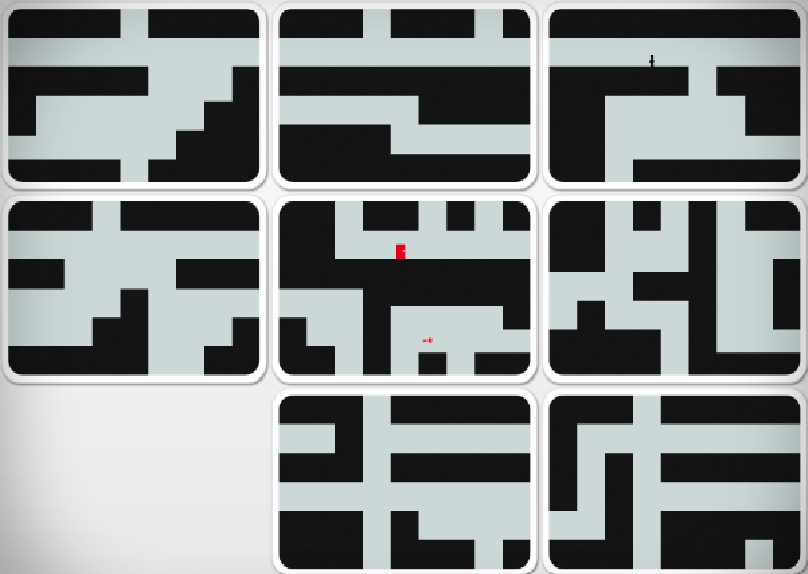
\includegraphics[scale=0.7]{resources/gui_original.png}
	  \end{center}
	
	A program felhasználói felületének tervezése során a felület kialakítását az egyszerűség és könnyen irányíthatóság irányelvei alakította ki. A menürendszer  felépítését az opciók minél gyorsabb elérésérére való törekvés határozta meg. Emiatt a játék közbeni lehetőségek mind elérhetőek egyetlen kattintással, vagy a megfelelő billentyű lenyomásával, gördülényebbé téve a játékmenetet. A fenti szempontok figyelembe vételével a felület látványterve:
	\begin{center}
		    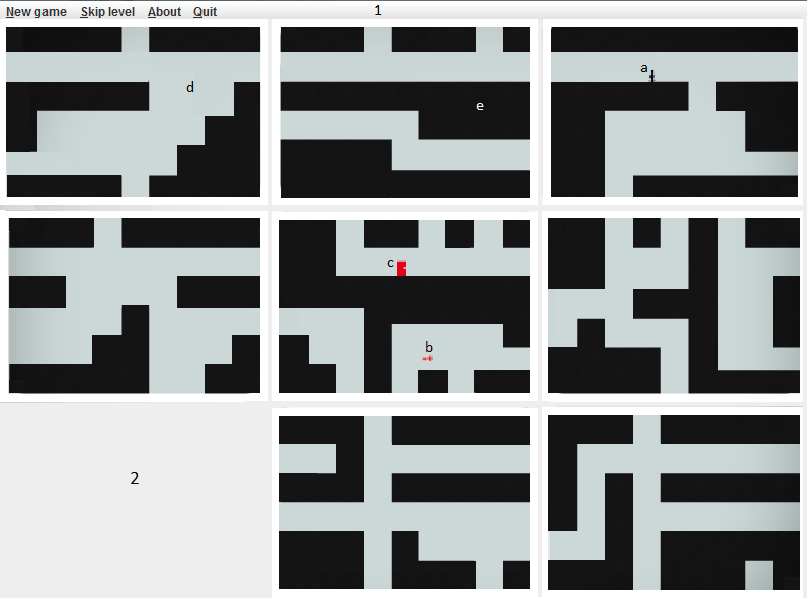
\includegraphics[scale=0.7]{resources/gui_own.png}
	 \end{center}
	 Az ábrán számokkal megjelölt kezelőelemek:
	 \begin{enumerate}
 \item Menüsáv
 		\begin{enumerate}
 		\item Menüsáv
 		\item Játéktér
		\end{enumerate}
 \item Játéktér
\end{enumerate}
1. 


		\subsection{A grafikus rendszer architektúrája}
		%A felület m űködésének elve, a grafikus rendszer architektúrája (struktúra diagramok). A struktúra diagramokon a prototípus azon és cs ak azon osztályainak  is szerepelnie kell, amelyekhez a grafikus felületet létrehozó osztályok kapcsolódnak.
		
		\subsubsection{A felület működési elve}
		%Le kell írni, hogy a grafikai megjelenésért felelős osztályok, objektumok hogyan kapcsolódnak a meglevő rendszerhez, a megjelenítés során mi volt az alapelv. Törekedni kell az MVC megvalósításra. Alapelvek lehetnek: push  alapú: a modell értesíti a felületet, hogy változott; pull  alapú: a felület kérdezi le a modellt, hogy változott-e;  kevert: a kett ő kombinációja.
		A grafikus felület a \texttt{Game} osztály által szolgáltatott publish/subscribe mintát megvalósító kommunikációs csatornán keresztül értesül a modell változásairól. A felület továbbá ismeri az aktuális \texttt{Game} objektumot, így téve lehetővé a játék állapotának megjelenítését. Amikor a modell megváltozik, ezen a csatornán egy \texttt{invalidate} esemény érkezik, melynek hatására a megjelenésért felelős osztályok újrarajzolják a grafikus felületet. Az újrarajzolás során a grafikus felület kérdezi le a \texttt{Game} osztály állapotát (melybe beleértendő az aktuális pálya állapota és a nézet), ami alapján a rajzolást végzi.
		
		\subsubsection{A felület osztály-struktúrája}
		%Osztálydiagram. Minden új osztály, és  azon régiek, akik az újakhoz közvetlenül kapcsolódnak.
			
	    \begin{center}
		    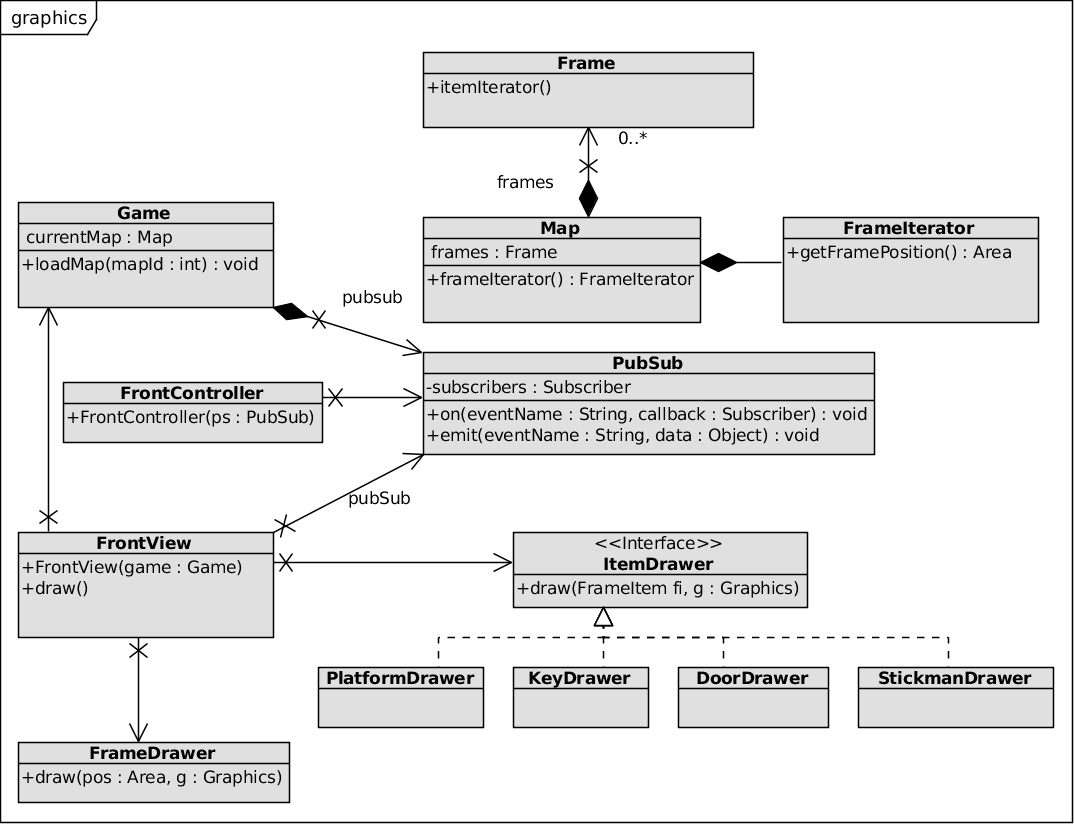
\includegraphics[scale=0.88]{resources/graphics.png}
	    \end{center}

	\subsection{A grafikus objektumok felsorolása}
	%Az új osztályok felsorolása. Az  régi osztályok közül azoknak a  felsorolása, ahol változás volt. Ezek esetén csak a változásokat kell leírni.	
	
	%GENERATOR:CLASS_DESCRIPTIONS
		\subsubsection{Osztály1}
			\begin{description}
				\item[Felelősség] Mi az osztály felel őssége. Kb 1 bekezdés. Ha szüks éges, akkor state-chart is.
				\item[Ősosztályok] Legősebb osztály → Ősosztály2  → Ősosztály3...
				\item[Interfészek] Mely interfészeket valósítja meg.
				\item[Attribútumok] Milyen attribútumai vannak
					\begin{description}
						\item[attribútum1] attribútum jellemzése: mire való, láthatósága (UML jelöléssel), típusa 
					\end{description}
				\item[Metódusok] Milyen publikus, protected és privát  metódus okkal rendelkezik. Metódusonként precíz leírás, 
ha szükséges, activity diagram is  a metódusban megvalósítandó algoritmusról.
					\begin{description}
						\item[int foo(Osztály3 o1, Osztály4 o2)] metódus leírása, láthatósága (UML jelöléssel)
					\end{description}
			\end{description}
	%GENERATOR:CLASS_DESCRIPTIONS

	\clearpage
	\subsection{Kapcsolat az alkalmazói rendszerrel}
	%Szekvencia-diagramokon ábrázolni kell a grafikus rendszer működését. Konzisztens kell legyen az el őz ő alfejezetekkel. Minden metódus,  ami ott szerepel, fel kell tűnjön valamelyik szekvenciában. Minden metódusnak, ami szekvenciában  szerepel, szereplnie kell a valamelyik osztálydiagramon.
		\subsubsection{Initialize}
		    \begin{center}
			    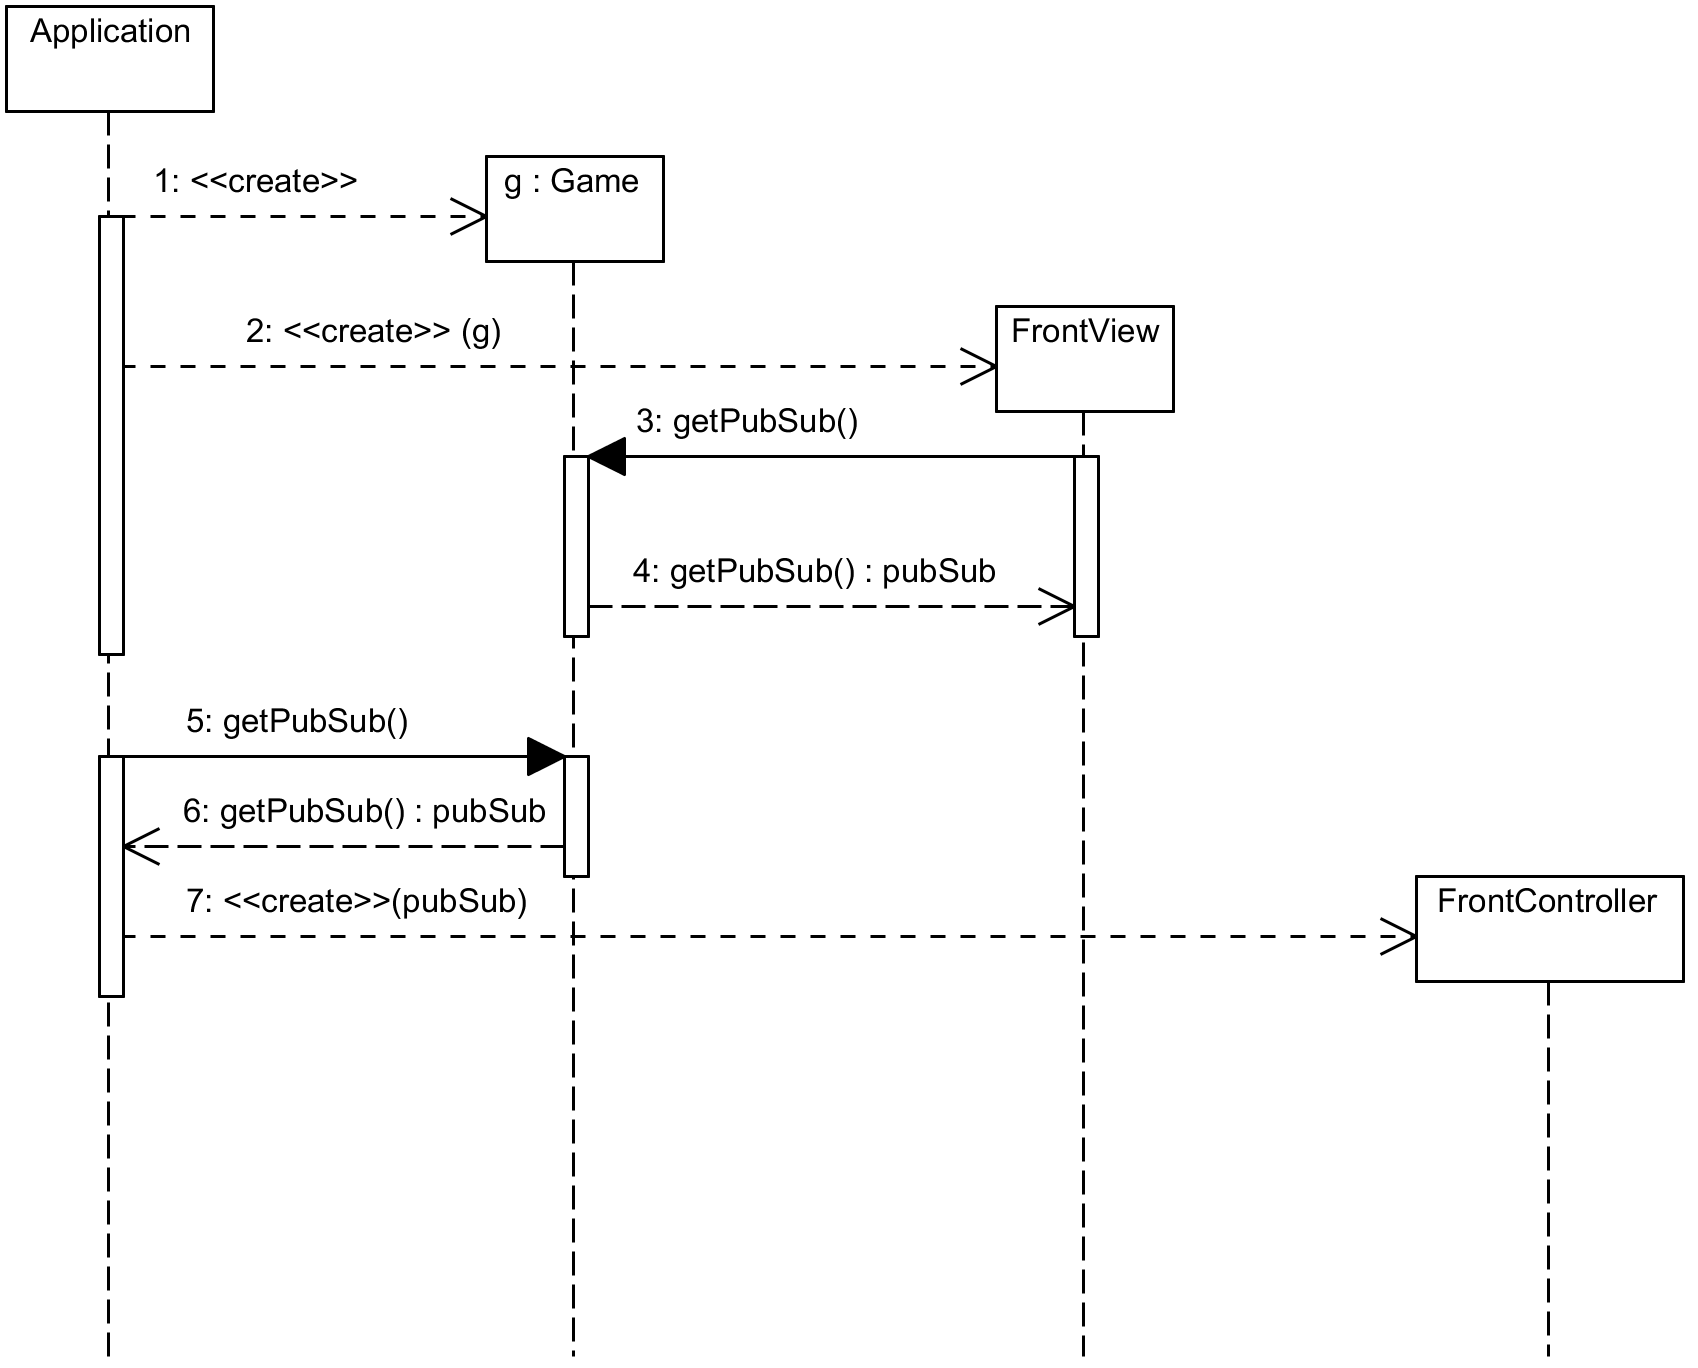
\includegraphics[scale=0.88]{resources/init.png}
		    \end{center}

		\subsubsection{Event}
		    \begin{center}
			    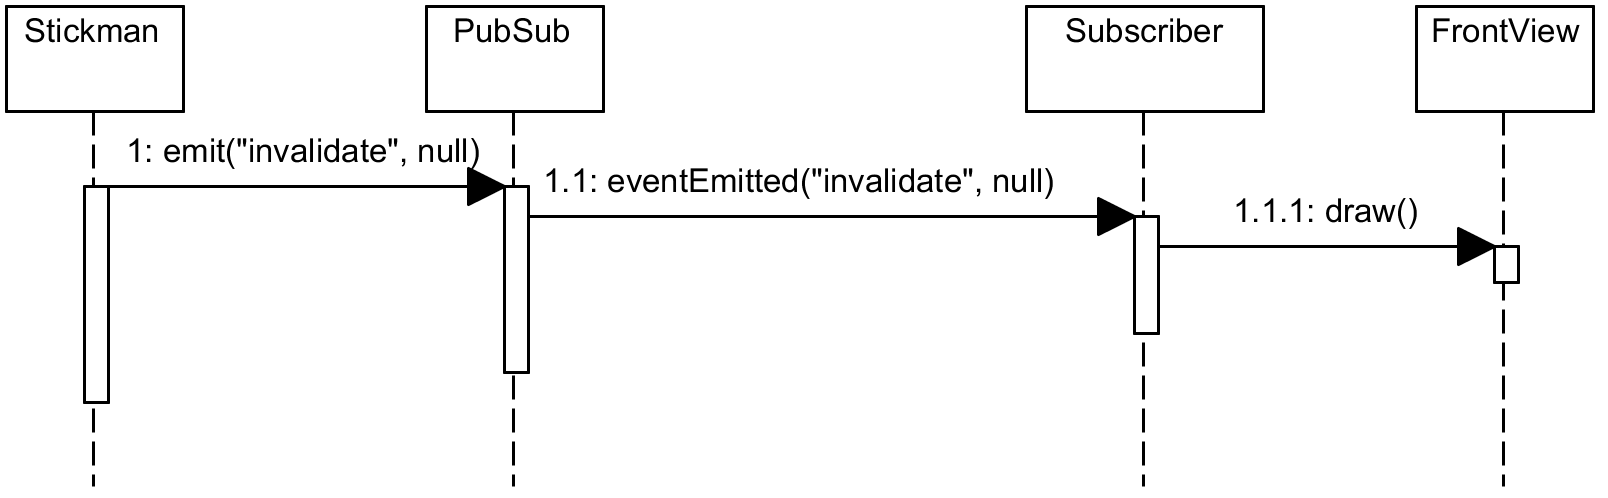
\includegraphics[scale=0.88]{resources/event.png}
		    \end{center}

		\subsubsection{Kirajzolás}
		    \begin{center}
			    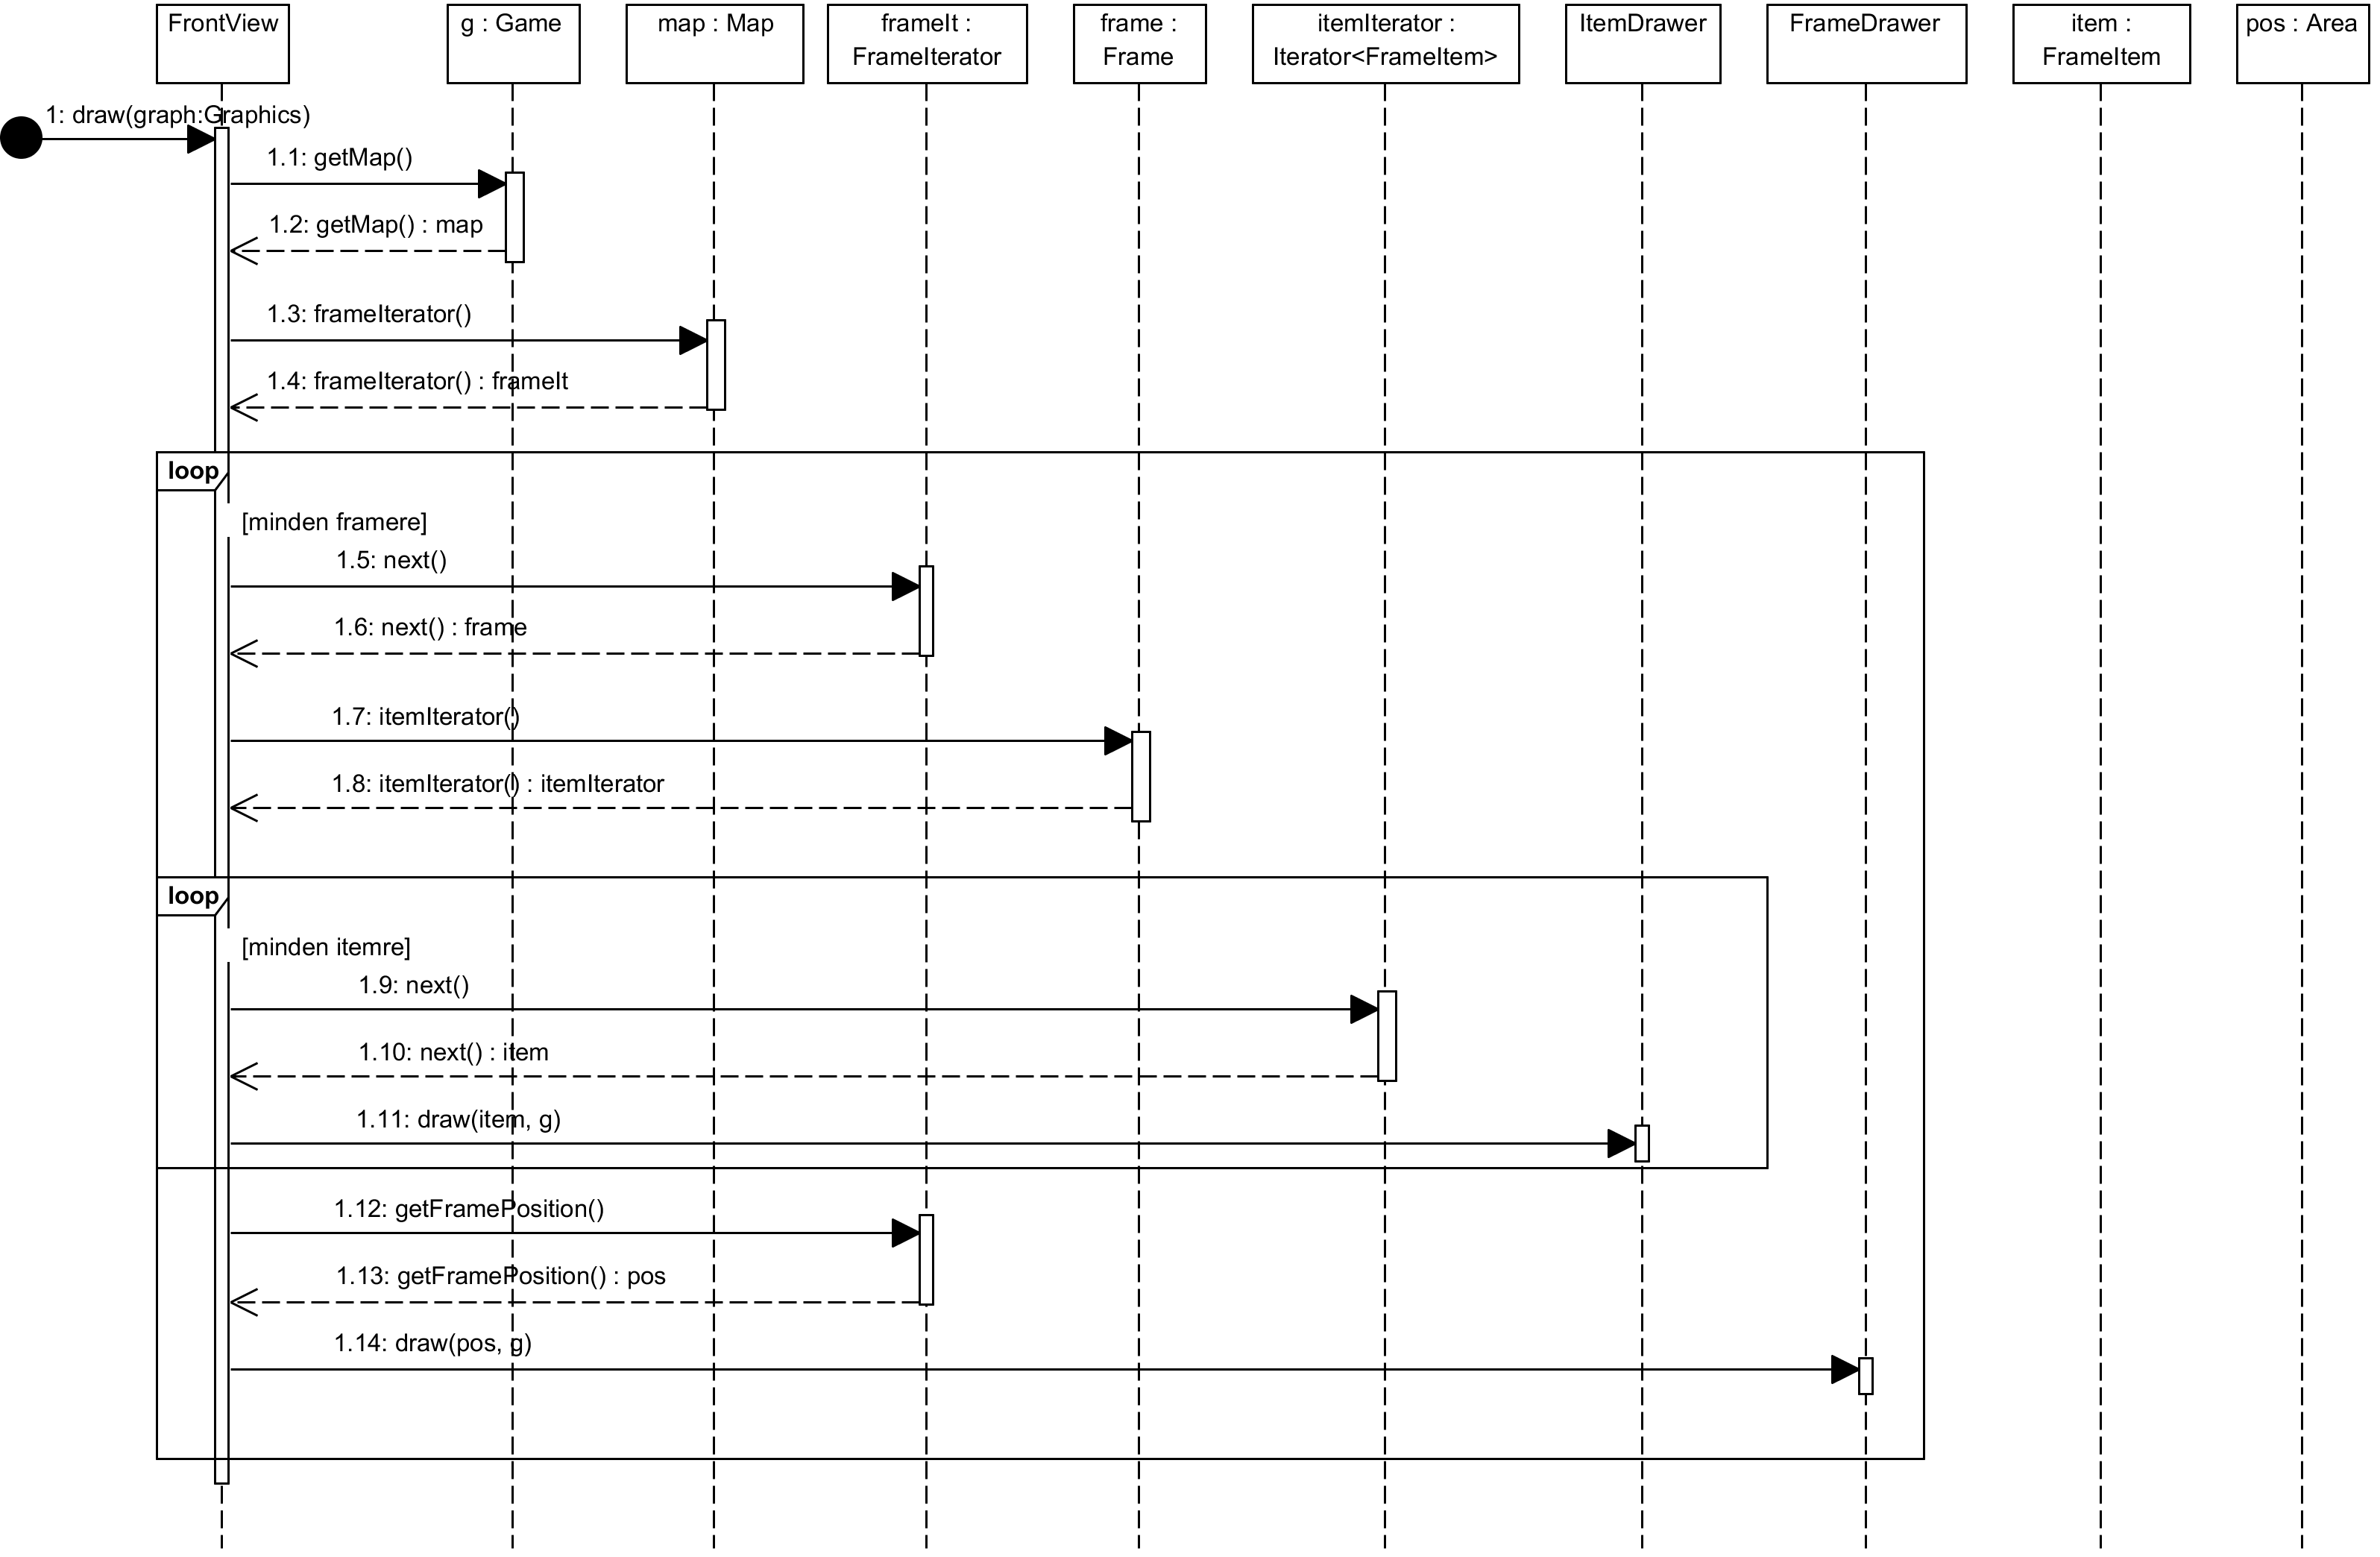
\includegraphics[scale=0.70, angle=-90]{resources/drawing.png}
		    \end{center}
	
		\subsection{Napló}
	% The diary generator uses the following comments to identify the beginning and the ending of the generated diary
	% The following content is auto generated, please do NOT modify, edit the related shared document instead.
	%GENERATOR:DIARY
	
	%GENERATOR:DIARY
\end{document}
